% document type
\documentclass [12pt, a4]{article} % oneside

% fixes
\usepackage{fixltx2e} % LaTeX patches, \textsubscript
\usepackage{cmap} % fix search and cut-and-paste in PDF

% language
\usepackage[english]{babel}
\usepackage[T1]{fontenc}
\usepackage[utf8]{inputenc}

% usability
\usepackage {float}

% formatting
\usepackage{amsmath}
\usepackage{amsfonts}
\usepackage{url}
\usepackage{setspace}
\usepackage{hyperref}

\usepackage{fancyvrb}
\usepackage{mdwlist}
\usepackage{float,caption}

\usepackage{graphicx}
\usepackage{ifpdf}
\usepackage{listings, textcomp, color, xcolor, caption}

\title{Approximating discontinous functions}

\author{
    Egon Elbre, Olga Agen \\
        Department of Computer Science \\
    University of Tartu\\
    Tartu\\
}

\date{\today}

\begin{document}

\maketitle

\begin{abstract}
Calculating discontinous functions can be difficult and computationally
expensive. By combining using approximation functions we can lower 
the computational expensiveness at the cost of errors.
Defining good approximation function can be a hard to get right. 
However, defining an approximation that works for some value can 
be simpler. We show how combining several simple approximations 
can give us a better approximation and reduce computational requirements.
\end{abstract}

\section{Introduction}

Calculating complex discontinous functions can be time consuming and finding good approximations can be difficult. In this report we propose a method that could be used to simplify finding of approximations. We show that composing several approximations can help us to achieve at a better approximation.


\paragraph{Outline}

We first describe how we can improve approximation functions if they 
satisfy some constraints. Then we show that we can allow some error
in satisfying these constraints. Then we show how to use it on 
calculating distances. Finally we show an approximation for
Levenshtein distance as an example.

\section{Improving approximations}

\newcommand{\Real}{\mathbb{R}}
\newcommand{\defas}{ := }
\newcommand{\err}[1]{\varepsilon_{#1}}

We are trying to approximate a function $f$:

$$f : X \mapsto \Real$$

Using $<$ we can define $\min$ and $\max$ for that set.

$$ \min(x,y) \defas \begin{cases}
    x & \text{if $x \leq y$}, \\
    y & \text{otherwise}.
\end{cases}
$$

$$
\max(x,y) \defas \begin{cases}
    y & \text{if $x \leq y$}, \\
    x & \text{otherwise}.
\end{cases}
$$

$X$ can be any set.

\subsection{Exact approximation}

Let's assume we are interested in range $R \subseteq X$. Let's assume we 
have functions $\alpha$ and $\beta$ such that

\begin{align*}
    \alpha(x) &\leq f(x), \forall x \in R \\
    \beta(x)  &\leq f(x), \forall x \in R 
\end{align*}

Now we can define $\epsilon$ function.

\begin{align*}
    \alpha(x) &= f(x) + \err\alpha, \err\alpha \geq 0 \\
    \beta(x)  &= f(x) + \err\beta, \err\alpha \geq 0
\end{align*}

It is trivial to derive function $\gamma$ where $\err\gamma$ is smaller 
than $\err\alpha$ and $\err\beta$.

\begin{align*}
    \gamma(x)   &= max(\alpha(x), \beta(x)) \\
                &= max(f(x) - \err\alpha(x), f(x) - \err\beta(x)) \\
                &= f(x) - min(\err\alpha(x), \err\beta(x)).
\end{align*}

This also gives us a usefulness requirement for $\alpha$ and $\beta$:

\begin{align*}
    \exists x \in R, ~ &\alpha(x) < \beta(x) \\
    \exists x \in R, ~ &\beta(x) < \alpha(x)
\end{align*}

This means that function $\alpha$ and $\beta$ must be complementary.
For some inputs one should give better approximations than the other.

\subsection{Probablisitic approximation}

Having such hard boundary severly restricts the possible functions we can
use. If we allow some mistake in the boundary we can get better precision,
but we may constrain our results.

\begin{align*}
    p_\alpha &\defas p(\alpha(x) \leq f(x)), x \in R \\
    p_\beta &\defas p(\beta(x)  \leq f(x)), x \in R 
\end{align*}

This means that the probability of error at place $x$ of the 
function $\gamma = max(\alpha, \beta)$ is:

$$ p_\gamma(x) = \begin{cases}
    p_\beta & \text{if $\alpha(x) \leq \beta(y)$}, \\
    p_\alpha & \text{otherwise}.
\end{cases}
$$

Probability of getting an error from the composite function:

$$
    max(p_\alpha, p_\beta) \leq p(\gamma(x) \leq f(x)) \leq p_\alpha + p_\beta
$$

\section{Distance approximation}

We can apply the same idea to distances:

$$
  \gamma(x,y) = max(\alpha(x,y), \beta(x,y))
$$

Since most distance measures are require pairwise computation over
a large set, it would be benefitial to decompose such functions.

$$
  \gamma(x,y) = max( dist_\alpha(t_\alpha(x), t_\alpha(y)), dist_\beta(t_\beta(x), t_\beta(y)) )
$$

This way we can reuse computation of $t_\alpha$ and $t_\beta$ or even do additional operations on it. For example it allows us to do range queries.

$$
  query(x,r) = \{ y | dist_\alpha(t_\alpha(x), t_\alpha(y)) <= r \} \cap \{ y | dist_\beta(t_\beta(x), t_\beta(y)) <= r \}
$$

If our distance function is simple, such as Manhattan or Euclidian, we can 
use advanced trees to store $t_\alpha$ and $t_\beta$ and use advanced query searches.

If we are working with probablistic approximations we could use fuzzy sets for 
results to have some error tolerance.

\section{Example: Levenshtein on Nucleotide Sequences}

As a starting point for designing approximation for Levenshtein distance
we picked Hamming distance\cite{wiki:Hamming}, Smoothing\cite{wiki:Smoothing}, Fourier tranformation\cite{wiki:Fourier} and Haar transformation\cite{wiki:Haar}.\footnote{We expect that reader is already familiar with these concepts.} The source code for the example can be found at "http://github.com/egonelbre/tranprox"\cite{Tranprox}.

\paragraph{Converting to signal}

One of the first problems is converting nucleotide sequence to a signal. There are multiple ways to do it. We chose tetrahedral representation as outlined in "Conversion of nucleotides sequences into genomic signals". \cite{cristea2002conversion}

Tetrahedral representation means each nucleotide is assigned to a tetrahedron corner. This means that the distance between any nucleotide is $1$ after conversion.

\paragraph{Transformation}

For transformation we use identity, smoothing, Fourier and Haar transformation.
If different length sequences are used then additional interpolation\cite{wiki:Interpolation} is required.


\paragraph{Distance}

As distance we use Euclidean and Manhattan distance. Euclidean has been modified to take into account complex numbers.

\paragraph{Normalization}

Since the distance between transformed data can be on different scale we somehow need to normalize. We chose a simple strategy:

$$f(x,y) - a*dist(t(x),t(y)) \geq 0$$
$$D = run(Q, t, dist) = \{ d ~ | ~ \forall x,y \in Q ~ d = f(x,y) / dist(t(x),t(y)) \}$$

Where $Q$ is some sample from the whole range $R$. Then we can use quantile function on $D$ to approximate the scaling. That way we allow some mistakes and minimize the error.

\paragraph{Measuring improvement}

We need to somehow approximate how much would an additional measure improve the previous measure. For that we use

\begin{align*}
D_{base} &= run(Q, t_{base}, dist_{base}) \\
D_{new} &= run(Q, t_{new}, dist_{new}) \\
improvement &= count(D_{base} > D_{new} ) / |Q|
\end{align*}

\paragraph{Dataset}

For evaluating methods we generated random dataset of 500 elements with 10 nucleotides per sequence.

\subsection{Hamming distance}

We use Hamming distance as our basis for our approximation.

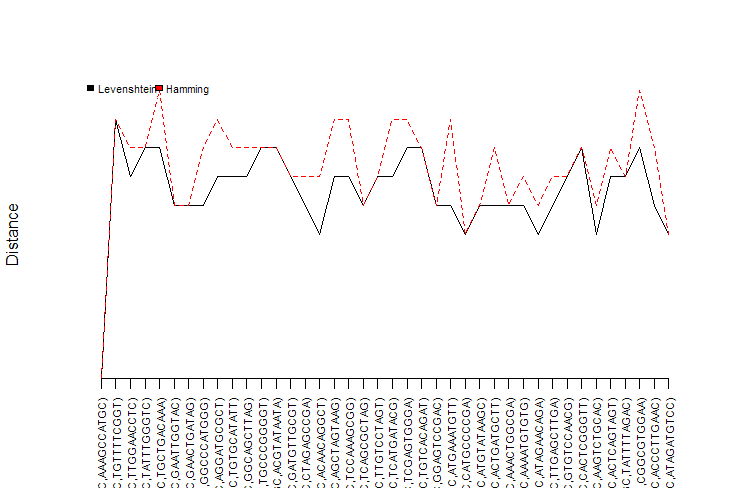
\includegraphics[width=0.9\textwidth]{img/hamming.png}

Here we can see that Hamming distance is an upper bound for Levenshtein distance.

\subsection{Fourier transformation}

We examine several variations of Fourier transformation and distance functions. First, we looked at fast Fourier transformation using at both Euclidean and Manhattan distances. We tried using only imaginary and only real parts of the FFT result and the combination.

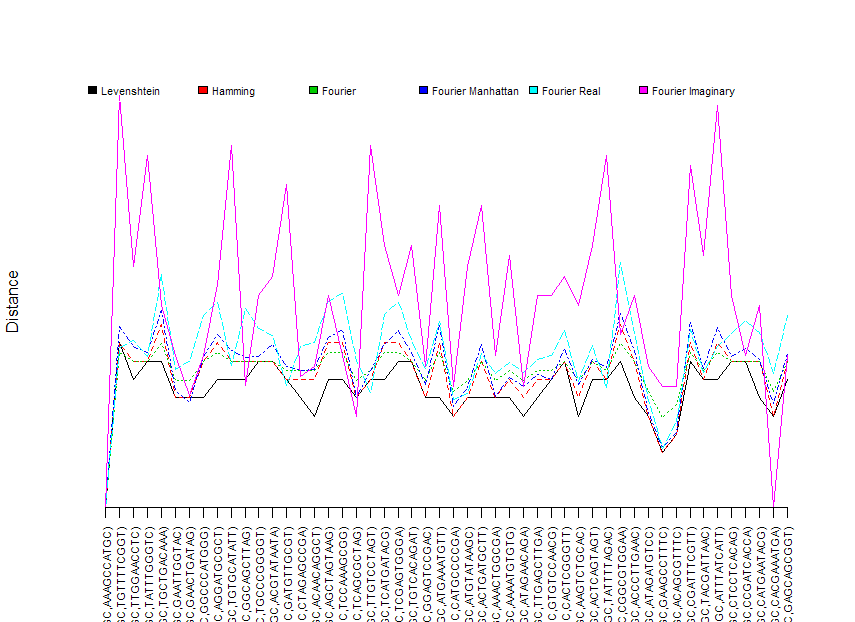
\includegraphics[width=0.9\textwidth]{img/fourier.png}

Fourier transformations provides some improvement to Hamming distance.

\begin{table}[H]
\begin{tabular}{ r | l }
    Transformation & Improvement \\ \hline
    Fourier           & 0.242712 \\
    Fourier Manhattan & 0.105872 \\
    Fourier Imaginary & 0.10732 \\
    Fourier Real      & 0.073592 \\
\end{tabular}
\end{table}

\subsection{Haar transformation}

We examine only Haar transformation from wavelet transformations. There are possibly other wavelets that give better improvement.

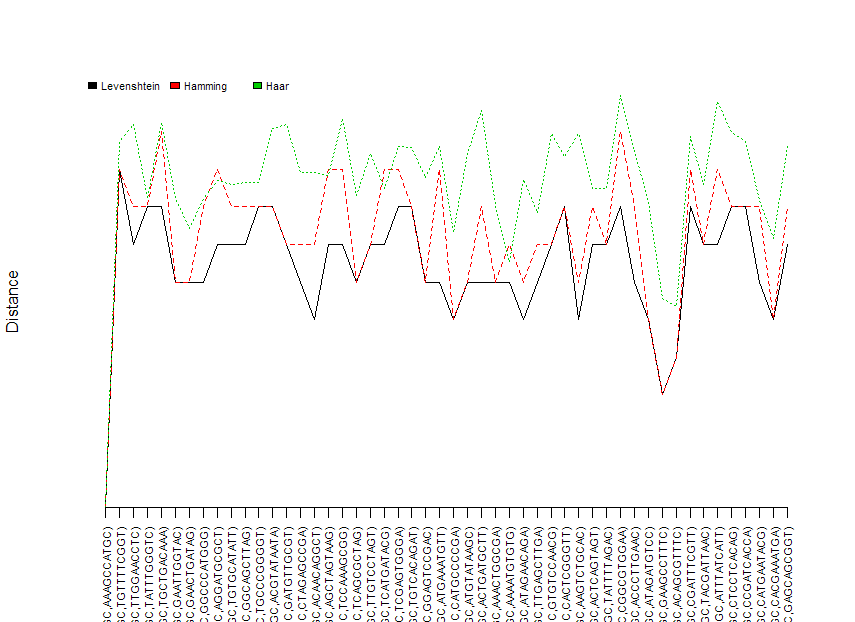
\includegraphics[width=0.9\textwidth]{img/haar.png}

Haar in this case improved by 0.142224.

\subsection{Smoothing transformation}

We use smoothing kernel $[1,2,1]$ for "Blur" and $[1,2,5,2,1]$ for "Blur5".

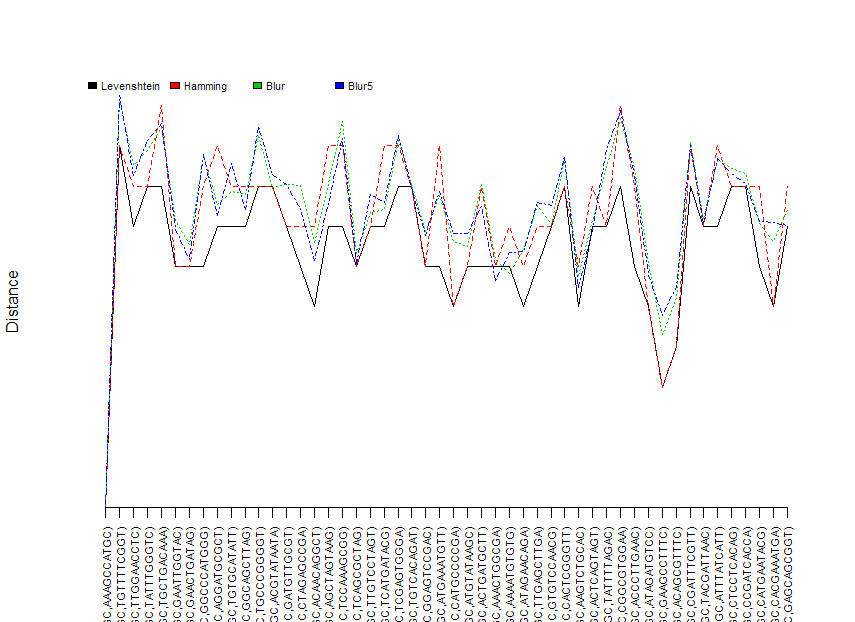
\includegraphics[width=0.9\textwidth]{img/blur.png}

The improvements are 0.422176 and 0.388 correspondingly.

\subsection{Composing}

We need to evaluate how to compose the transformations to get the best approximation.

We choose to compose the best transformations first (Hamming, Blur). Then Fourier and Haar do not give any improvement to that composition. In Levenshtein case we can do additionally "floor" operation because we know that the transformed distance must be larger than Levenshtein and Levenshtein can only have integer values.

\subsection{Queries}

To validate how well this function composing works we first generated 3000 DNA sequences and 100 query sequences. Then we queried using different ranges using both the composite and levenshtein distance.

This table shows sensitivity:

\begin{table}[H]
\centering
\begin{tabular}{ r | l l l }
Method / Range & 3 & 4 & 5 \\ \hline
Composed & 0.7495817 & 0.6649334 & 0.6781805 \\
Hamming  & 0.5794757 & 0.4675806 & 0.4433428 \\
Blur     & 0.4545455 & 0.4823919 & 0.5315241 \\
\end{tabular}
\end{table}

This table shows false discovery rate:

\begin{table}[H]
\centering
\begin{tabular}{ r | l l l }
Method / Range & 3 & 4 & 5 \\ \hline
Composed & 0.1913357 & 0.1484209 & 0.1024433 \\
Hamming  & 0         & 0         & 0         \\
Blur     & 0.2806708 & 0.1937056 & 0.127116  \\
\end{tabular}
\end{table}

We can see false discovery rate and sensitivity drop as we increase the range.
We can see that the composed method is more sensitive than uncomposed versions.
Also the composed functions FDR is between Hamming and Blur methods.

\section{Results}

We have examined the basic foundations of composing approximate functions and shown
how one would proceed to design better approximations. We also showed that
the composed approximation is better than the simple approximations.

We learned that the design of approximationing functions becomes much simpler 
when we restrict the space where they must work correctly.

We were unable to investigate the performance improvements due to time constraints. 

This preliminary research on this methodology of composing approximate functions gives
some confirmation that it can be useful. The extent of usability needs further analysis.

\nocite{*}
\bibliographystyle{ieeetr}
\bibliography{bibliography}

\end{document}